\chapter{Background}\label{ch:etichtta}
In questo capitolo verranno presentati i concetti teorici necessari per la comprensione della botnet Mirai e delle tecniche che essa impiega per andare a compromettere i dispositivi e coordinarne le attività.
\newline Si partirà da una panoramica generale sul concetto di botnet, analizzandone la struttura e i modelli di comunicazione. Successivamente si introdurranno i dispositivi IoT per capire come la loro sicurezza ridotta abbia permesso un'espansione così grande della botnet Mirai. Infine verranno analizzati tutti gli aspetti della botnet Mirai tra cui l'architettura, la modalità di propagazione, le capacità offensive della botnet e il malware che ha permesso la sua implementazione.
\section{Le botnet}
Una botnet, abbreviazione di \emph{robot-network}, è una rete di dispositivi compromessi sotto il controllo di un attore malevolo, chiamato \emph{bot-master}, che li utilizza per attacchi di vario tipo \cite{info_botnet}. L'architettura di una botnet è composta dai bot, rappresentati dai dispositivi compromessi, e da un server \emph{Command and Control} (CNC) utilizzato per inviare istruzioni ai bot \cite{architettura_botnet}. Si distinguono due principali modelli di botnet, i quali si differenziano principalmente per il metodo di comunicazione tra i bot e il CNC, e sono \cite{architettura_botnet}:
\begin{itemize}
    \item \textbf{Modello centralizzato}: botnet guidate da un solo server CNC, il quale da solo invia le istruzioni a tutti i bot, ciò implica che se il server CNC viene scoperto è a rischio l'intero funzionamento della botnet. Questo rende il modello centralizzato molto vulnerabile ad azioni di mitigazione;
    \item \textbf{Modello decentralizzato}: anche chiamato modello \emph{peer-to-peer } (P2P), in questo caso anche i bot possono inviare le istruzioni generate inizialmente dal bot-master. Quindi fin quando quest'ultimo riesce a comunicare con un solo bot il funzionamento della botnet non è compromesso, tutto ciò rende questo modello più resistente ad azioni di mitigazione.

\end{itemize}
Nella Figura~\ref{botnet_centr_p2p} vengono rappresentati il modello centralizzato e il modello decentralizzato mostrando come il modello decentralizzato sia più resiliente rispetto a quello centralizzato.
\begin{figure}[H]
    \centering
    \includegraphics[width=0.75\linewidth]{tesi_stile/img/botnet_centr_p2p.png}
    \caption{Modello centralizzato e decentralizzato \cite{mod_centr_decentr}.} 
    \label{botnet_centr_p2p}
\end{figure}
La costruzione di una botnet segue tipicamente queste fasi sequenzialmente \cite{architettura_botnet}:
\begin{enumerate}
    \item \textbf{Infezione}: l'attaccante sfrutta una vulnerabilità per esporre i dispositivi ad un malware. La vulnerabilità oltre che nel sistema può anche trovarsi anche nel comportamento umano, l'obiettivo è quello di esporre l'utente inconsapevole all'infezione del malware. Solitamente gli attaccanti sfruttano i problemi di sicurezza dei software e/o degli hardware oppure inviano il malware tramite e-mail o altri messaggi online;
    \item \textbf{Iniezione}: la vulnerabilità precedentemente trovata viene utilizzata per infettare il sistema eseguendo il codice malevolo; 
    \item \textbf{Connessione}: il dispositivo compromesso attraverso l'esecuzione di codice malevolo apre un connessione con il server CNC diventando effettivamente un bot sotto il controllo del bot-master. I bot a loro volta possono eseguire una scansione della rete alla ricerca di dispositivi vulnerabili, l'obiettivo finale è quello di controllare il maggior numero di dispositivi possibile in modo da disporre di un'enorme potenza di attacco;
    \item \textbf{Esecuzione di attività malevole}: i bot possono essere istruiti dal bot-master per svolgere una serie di attività malevole;
    \item \textbf{Mantenimento}: il bot-master utilizza differenti metodi per mantenere attiva la botnet. Tra cui l'aggiornamento e l'eliminazione di bot sospetti o non più attivi.
\end{enumerate}
Il numero di dispositivi infettati da una botnet può raggiungere centinaia di migliaia di unità. Una volta che la botnet è attiva essa può portare a termine una serie di attività malevole tra le quali \cite{attività_malevole}:
\begin{itemize}
    \item \textbf{Distributed Denial-of-Service (DDoS)}: i bot vengono utilizzati per generare un enorme quantità di traffico di rete verso siti web o altri servizi con lo scopo di interromperne la disponibilità per un tempo più o meno lungo;
    \item \textbf{Campagne di Phishing}: vengono imitate identità o organizzazioni fidate per indurre gli utenti a divulgare informazioni riservate. In questo caso i bot vengono impiegati nell'invio di messaggi di spam volti al furto di credenziali di accesso a servizi di vario genere e alla distribuzione di malware di ogni tipo;
    \item \textbf{Mining di criptovalute}: viene utilizzata la potenza computazionale aggregata della botnet;
    \item \textbf{Affitto della botnet}: tramite il modello \emph{Botnet-as-a-Service} si può concedere, previo pagamento, l'utilizzo della botnet per scopi malevoli a terze parti.
    
\end{itemize}
\subsection{Botnet IoT}
I dispositivi candidati ad essere parte di una botnet sono tutti quelli in grado di connettersi a internet, quindi non solo computer e smartphone ma anche quei dispositivi che fanno parte dell'\emph{Internet of Things} (IoT). Questo termine si riferisce a tutti quei dispositivi che sono in grado di raccogliere, memorizzare ed inviare informazioni attraverso la rete come ad esempio smart TV, smartwatch, elettrodomestici smart, veicoli, telecamere di sicurezza, macchinari industriali e sensori. I vantaggi dell'ecosistema IoT sono i seguenti \cite{iot_vantaggi}:
\begin{itemize}
    \item \textbf{Efficienza}: molte attività vengono automatizzate permettendo un notevole risparmio di tempo;
    \item \textbf{Riduzione dei costi}: la produzione di beni e servizi potrebbe richiedere minore intervento umano, questo si traduce in un costo minore per il consumatore finale;
    \item \textbf{Controllo qualità}: le attrezzature IoT, soprattutto quelle industriali, favoriscono una migliore comunicazione tra dispositivi permettendo un maggior controllo della qualità.
    
\end{itemize}
Per questo motivo l'IoT è in costante crescita infatti vengono creati nuovi dispositivi in continuazione, tali dispositivi però possono avere una serie di problemi \cite{iot_svantaggi}:
\begin{itemize}
    \item \textbf{Sistemi operativi obsoleti}: i dispositivi IoT presentano sistemi operativi vecchi con vulnerabilità note che possono essere tranquillamente sfruttate da un attaccante per violare la sicurezza del dispositivo. Questi sistemi operativi vecchi vengono installati poiché i dispositivi IoT molto spesso non hanno risorse necessarie per supportare sistemi operativi moderni;
    \item \textbf{Mancanza di sicurezza integrata}: a differenza dei computer tradizionali, che molto spesso presentano sistemi antivirus e di rilevamento delle intrusioni (IDS) integrati, i dispositivi IoT non offrono lo stesso livello di protezione risultando più facili da compromettere;
    \item \textbf{Aggiornamenti non frequenti}: tutti i software vengono aggiornati periodicamente sia per aggiungere funzionalità sia per risolvere bug di sicurezza. I dispositivi IoT ricevono gli aggiornamenti molto meno frequentemente esponendoli ad attacchi mirati;
    \item \textbf{Credenziali deboli}: i dispositivi IoT presentano una serie di problemi legati alla sicurezza delle credenziali. I produttori molto spesso distribuiscono i loro prodotti con credenziali predefinite e non impongono agli utenti di modificarle, in questo scenario un attaccante con un semplice attacco \emph{brute-force} potrebbe accedere al dispositivo;
    \item \textbf{Utilizzo di protocolli deprecati}: alcuni protocolli, come Telnet, non vengono più utilizzati a causa della loro scarsa sicurezza. Tuttavia alcuni dispositivi IoT continuano ad utilizzarli mettendo a rischio la sicurezza dei dati dell'utente.
\end{itemize}
Nella Figura~\ref{IoT_crescita} viene mostrata come il mercato dei dispositivi IoT sia in continua crescita mettendo in luce come la sicurezza di questi dispositivi sia un elemento imprescindibile al giorno d'oggi.
\begin{figure}[H]
    \centering
    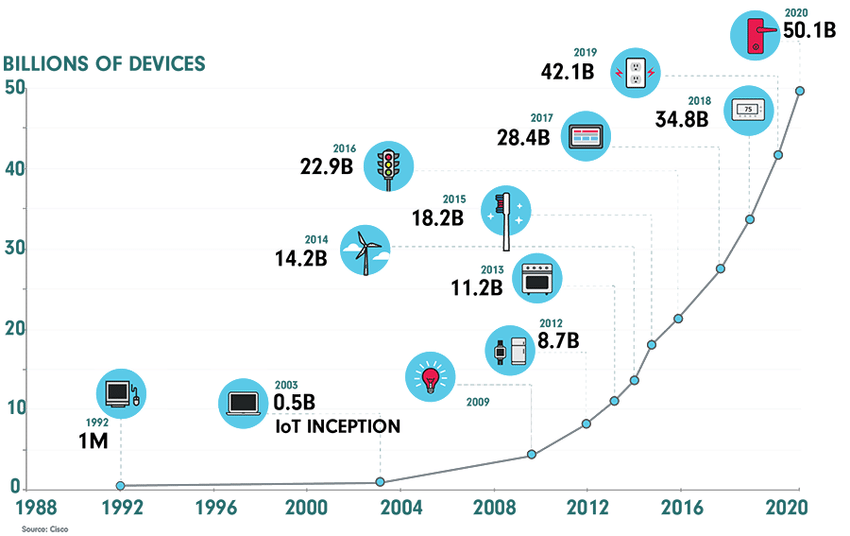
\includegraphics[width=0.75\linewidth]{tesi_stile/img/IoT_crescita.png}
    \caption{Crescita dei dispositivi IoT \cite{IoT_grafico}.}
    \label{IoT_crescita}
\end{figure}
Le debolezze nei dispositivi IoT possono essere sfruttate per accedere a quest'ultimi ed eseguire del codice malevolo. Una volta fatto ciò i dispositivi possono essere controllati da remoto dando vita ad una botnet IoT e possono essere istruiti ad esempio per andare ad eseguire un attacco DDoS verso un server bersaglio. In questo contesto si inserisce Mirai, un malware che accede ai dispositivi IoT sfruttando le credenziali deboli, che ha dato vita ad una delle più grandi botnet IoT mai esistite.
\section{Attacchi DoS/DDoS}
Come detto in precedenza uno degli scopi per cui le botnet vengono create è quello di lanciare attacchi DDoS. Quest'ultimi non sono altro che un'estensione degli attacchi DoS (Denial-of-Service), una tipologia di attacco attraverso il quale viene inondato di richieste un servizio degradandone, o nei casi più gravi interrompendone, la disponibilità. Un attacco DDoS (Distributed Denial-of-Service) segue lo stesso principio, con l'unica differenza che il traffico massivo è generato da una moltitudine di macchine compromesse, organizzate all'interno di una botnet. Questo rende l'attacco DDoS difficile da mitigare e molto più insidioso di un attacco DoS tradizionale. Le principali tipologie di attacchi DDoS si suddividono in tre categorie principali e ciascuna coinvolge diversi livelli della rete descritti nel modello OSI (Open System Interconnection)\footnote{ISO/IEC 7498-1:1994. \url{https://www.iso.org/standard/20269.html}}. Tra questi attacchi possiamo distinguere l'attacco volumetrico, l'attacco basato sul protocollo e l'attacco a livello applicativo. Di seguito ciascuna di esse verrà descritta nel dettaglio \cite{ddos_info}: 
\begin{itemize}
    \item \textbf{Attacco volumetrico}: in questa tipologia di attacco l'attaccante tenta di saturare tutta la larghezza di banda tra Internet e il bersaglio, impedendo agli utenti legittimi di usufruire del servizio colpito. Gli attacchi DDoS volumetrici sono noti per sovraccaricare le misure che vengono attuate per mitigare gli attacchi DDoS stessi. Tra le varianti più comuni rientrano: gli \emph{UDP flood}, gli \emph{ICMP flood} e gli attacchi di amplificazione DNS. Prendendo come esempio quest'ultimi, l'attaccante invia utilizzando un indirizzo IP contraffatto ,appartenente alla vittima,  richieste di \emph{lookup} al server DNS. Queste richieste chiedono di restituire una grande quantità di informazioni per ognuna di esse. Il server DNS quindi risponderà ad ogni richiesta inondando di dati l'indirizzo IP della vittima; 
    \item \textbf{Attacco a livello applicativo}: questo attacco prende di mira le applicazioni di una rete che nel modello OSI rientrano nel livello 7. Gli attacchi di questo tipo bersagliano siti e applicazioni web interrompendone la disponibilità e non permettendo ad un utente legittimo di utilizzarli. La forma più comune di attacco a livello applicativo è l'\emph{HTTP flood}, in questo attacco l'attaccante utilizza più dispositivi per inviare molteplici richieste HTTP ad un sito web. Il server bersaglio non riuscendo a gestire tutte le richieste rallenta o nei casi peggiori interrompe completamente il servizio;
    \item \textbf{Attacchi al protocollo}: questi attacchi prendono di mira il livello di rete e il livello di trasporto ovvero il livello 3 e 4 del modello OSI. Gli attacchi al protocollo, noti anche come attacchi di esaurimento dello stato, causano un'interruzione della disponibilità per via dell'esaurimento delle risorse del server e/o dei dispositivi intermedi come firewall e bilanciatori di carico. Un attacco tipico che rientra in questa categoria è l'attacco \emph{smurf}. Quest'ultimo utilizza l'ICMP (Internet Control Message Protocol), ovvero un protocollo per diagnosticare lo stato di comunicazione tra due dispositivi. In uno scambio ICMP tipico, un dispositivo invia una richiesta ICMP di tipo \emph{echo} ad un altro dispositivo il quale risponde in modo analogo. In un attacco smurf l'attaccante inoltra una richiesta echo ICMP  ad un indirizzo di rete \emph{broadcast}, falsificando il suo indirizzo IP con quello della vittima. I dispositivi che ricevono la richiesta rispondono simultaneamente all'indirizzo IP della vittima, generando un enorme volume di traffico così da saturarne rapidamente le risorse. Questo attacco a differenza degli altri DDoS non richiede l'utilizzo di una botnet. Nella Figura~\ref{grafico_DDoS} è mostrato l'andamento temporale di un attacco HTTP flood registrato nel 2016 da Cloudflare e attribuito a una botnet IoT, probabilmente Mirai o qualche sua variante. L'attacco ha coinvolto circa 52000 indirizzi IP e ha raggiunto un picco di 1.75 milioni di richieste al secondo (Mrps).
    
\end{itemize}
\begin{figure}[H]
    \centering
    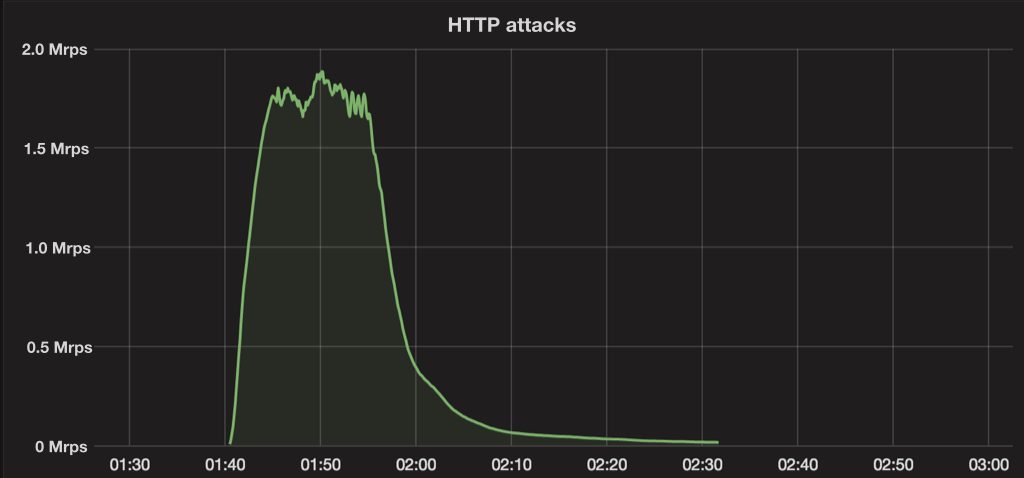
\includegraphics[width=0.75\linewidth]{tesi_stile/img/grafico_DDoS.png}
    \caption{Andamento di un attacco HTTP flood (livello 7) \cite{grafico_DDoS_cit}.}
    \label{grafico_DDoS}
\end{figure}


\section{Il malware Mirai}
Mirai è un malware di tipo \emph{worm-like}, progettato per compromettere dispositivi IoT e trasformarli in bot controllati da remoto, organizzati in una botnet ed utilizzati per eseguire attacchi DDoS su larga scala, con lo scopo di degradare la disponibilità di servizi online, siti web o intere infrastrutture di rete. Mirai è stato programmato da tre giovani di nome Paras Jha, Dalton Norman e Josiah White \cite{dip_giustizia} per attaccare server rivali su Minecraft, invitando successivamente le vittime a pagare per evitare ulteriori interruzioni del servizio e dando così avvio a un vero e proprio racket di protezione. Il codice di Mirai, scritto nel linguaggio C e progettato per essere compatibile con diverse architetture utilizzate nei dispositivi IoT, divenne open-source quando un utente noto come  ``Anna-Senpai'', pseudonimo che gli investigatori riconducono a Paras Jha \cite{colpevolezza}, lo ha pubblicato su un forum chiamato ``Hackforums'' a settembre del 2016 \cite{post_originale_mirai}. Da questo momento in poi il codice sorgente di Mirai è stato utilizzato come base per la creazione di numerose altre botnet composte da dispositivi IoT, come dimostrano le molteplici varianti identificate successivamente. Questa pubblicazione ha permesso inoltre a persone con una minima abilità informatica di replicare facilmente la botnet Mirai.
La combinazione di questi fattori portò, alla fine del 2016, al rilevamento di attacchi DDoS su larga scala, in particolare fu lanciato un attacco al web host OVH che raggiunse 1 Tbit/s successivamente fu anche riportato un attacco al sito ``Krebs on Security'' che raggiunse i 620 Gbit/s \cite{info_mirai}.
L'attacco più importante però si verificò il 21 ottobre 2016 quando venne lanciato un DDoS contro Dyn, oggi Oracle Dyn un noto fornitore di servizi DNS, che interruppe la disponibilità di servizi come Github, Netflix, Reddit, Twitter e altri ancora \cite{attacchi_mirai}. Poco dopo toccò alla già debole infrastruttura Internet della Liberia, la quale subì un attacco DDoS che impedì l'accesso ad Internet per alcuni giorni \cite{attacchi_mirai}.
Nel dicembre del 2017 Paras Jha, Dalton Norman e Josiah White ammisero la loro colpevolezza dichiarando di aver infettato oltre 300000 dispositivi IoT per usarli in attacchi DDoS \cite{dispositivi_infettati}. Secondo l’accordo di patteggiamento, Paras Jha ammise di aver scritto il codice sorgente di Mirai intorno al luglio 2016 e di averlo utilizzato, insieme ai suoi complici, per colpire con attacchi DDoS diversi bersagli \cite{dispositivi_infettati}. Nella Figura~\ref{timeline_Mirai} viene mostrata una timeline raffigurante gli eventi principali riguardanti la botnet Mirai.
\begin{figure}[H]
    \centering
    \includegraphics[width=0.75\linewidth]{tesi_stile/img/timeline_Mirai.png}
    \caption{Timeline della botnet Mirai.}
    \label{timeline_Mirai}
\end{figure}

Ad oggi, nonostante siano passati quasi dieci anni dalla pubblicazione del codice sorgente, continuano a essere scoperte varianti di Mirai come Satori, Mukashi, Moobot e Sonic, le quali condividono parte del codice originale e si differenziano principalmente per le vulnerabilità sfruttate e per le tipologie di dispositivi presi di mira \cite{varianti_Mirai}.
Questo dimostra che Mirai ha avuto e continua ad avere un ruolo centrale nella creazione delle botnet orientate a dispositivi IoT, per comprenderne il funzionamento bisogna necessariamente descriverne le componenti interne e i meccanismi operativi che la caratterizzano.



\subsection{Architettura di Mirai}
La botnet Mirai, così come pensata dai suoi creatori, si basa su un modello centralizzato le cui componenti sono rappresentate da \cite{mirai_desc_architettura}:
\begin{itemize}
    \item \textbf{CNC server}: componente centrale della botnet utilizzata per andare ad istruire i bot, avviando così attacchi DDoS verso specifici bersagli. I bot e gli utenti autorizzati ad utilizzare la botnet sono memorizzati all'interno di un database MySQL gestito da uno o più admin;
    \item \textbf{Bot}: dispositivi compromessi che vengono controllati in modalità remota dall'attaccante, svolgono anche la funzione di scanner alla ricerca di nuovi dispositivi infettabili;
    \item \textbf{Report server}: fornisce informazioni riguardanti nuovi dispositivi potenzialmente infettabili al loader server;
    \item \textbf{Loader server}: esegue il malware sui dispositivi ricevuti dal report server.
\end{itemize}
Il Listato~\ref{setup_mirai} riporta un estratto del post pubblicato dall'utente ``Anna-Senpai'' insieme al codice sorgente, nel quale viene descritta la configurazione dell'infrastruttura utilizzata per la botnet \cite{post_originale_mirai}. Nella configurazione originale (``Pro Setup''), come riportato nel Listato~\ref{setup_mirai}, di Mirai sono state adoperate 4 macchine separate, precisamente 1 macchina per il server CNC e 3 macchine NFOrce\footnote{{\url{https://www.nforce.com/}}} per il loader server. Inoltre sono stati utilizzati 2 VPS\footnote{\url{https://www.ibm.com/think/topics/vps}} (Virtual Private Server) per ospitare il database MySQL e il report server. Nello stesso post viene proposta una soluzione alternativa che riduce al minimo il numero di server necessari per la creazione della botnet. In questa configurazione (``Bare Minimum'') il server CNC viene accorpato con il database MySQL e vengono utilizzate una macchina per il report server ed una o più macchine per il loader server.
\begin{lstlisting}[caption={Configurazione della botnet proposta dall'autore ``Anna-Senpai'' .}, label={setup_mirai}]
    Pro Setup (my setup)
    2 VPS and 4 servers
    - 1 VPS with extremely bulletproof host for database server
    - 1 VPS, rootkitted, for scanReceiver and distributor
    - 1 server for CNC (used like 2% CPU with 400k bots)
    - 3x 10gbps NForce servers for loading (distributor distributes to 3 servers equally)
\end{lstlisting}
Nella Figura~\ref{architettura_mirai} è illustrata l'architettura della botnet Mirai con i suoi attori principali e le operazioni svolte da ogni componente coinvolta, mostrando come i server e i bot lavorano in modo coordinato per compromettere quanti più nuovi dispositivi possibili.
\begin{figure}[H]
    \centering
    \includegraphics[width=0.75\linewidth]{tesi_stile/img/mirai_architecture.png}
    \caption{Architettura della botnet Mirai \cite{architettura_mirai}.}
    \label{architettura_mirai}
\end{figure}
\subsection{Propagazione di Mirai } 
La botnet Mirai si propaga infettando nuovi dispositivi IoT, per fare ciò esegue questi passaggi sequenzialmente sfruttando le credenziali deboli di quest'ultimi: 
\begin{enumerate}
    \item \textbf{Ricerca di dispositivi vulnerabili}: i bot eseguono una scansione massiva di Internet utilizzando indirizzi IP generati in modo casuale da una funzione interna, da questo processo vengono esclusi alcuni intervalli di indirizzi IP  riservati ad utilizzi particolari, come ad esempio l'indirizzo \emph{localhost} e l'indirizzo \emph{multicast}, oltre agli indirizzi IP associati ad infrastrutture sensibili quali il servizio postale e il Dipartimento della Difesa statunitensi \cite{attacchi_mirai}. Durante questa scansione si tenta, tramite un approccio \emph{brute-force}, un accesso sulla porta TCP 22 o TCP 23, utilizzate rispettivamente da SSH e Telnet, provando circa 60 coppie di credenziali deboli comunemente impostate dai produttori \cite{attacchi_mirai}. Una volta che l'accesso tramite SSH o Telnet va a buon fine, il bot riporta al report server l'avvenuta compromissione \cite{attacchi_mirai}. Nel Listato~\ref{combinazioni_comuni} sono illustrate alcune delle combinazioni username/password che durante la fase di scansione di Mirai vengono provate per accedere ai dispositivi individuati \cite{mirai_password_provate}. La lista completa delle credenziali che vengono testate è illustrata nell'Appendice~\ref{all_credenziali_provate}.
    \begin{lstlisting}[caption={Alcune combinazioni username/password provate.}, label={combinazioni_comuni}]
    // root     admin
    // admin    admin
    // root     888888
    // root     xmhdipc
    // root     default
    // root     juantech
    // root     123456
    // root     54321
    // support  support
    // root     (none)
    // admin    password
    // root     root
    // root     12345
    // user     user
    // admin    (none)
    // root     pass
    // admin    admin1234
    \end{lstlisting}

    \item\textbf{Infezione dei dispositivi vulnerabili}: visto che i dispositivi IoT hanno architetture diverse, ad esempio ARM, MIPS, x86, SPC e altre, il loader server dispone di binari compilati tramite dei \emph{cross-compiler}. Un \emph{cross-compiler} è un compilatore in grado di generare eseguibili per un'architettura diversa da quella su cui viene compilato. Il loader server rimane in ascolto delle informazioni inviate dal report server, che includono l’indirizzo IP, lo username, la password e la porta del dispositivo vulnerabile. Per eseguire contemporaneamente il malware sui dispositivi vulnerabili ricevuti, il loader server crea un insieme di \emph{worker}, ovvero thread che processano le informazioni sui dispositivi individuati come vulnerabili e si occupano di infettarli. In particolare, un \emph{worker}, una volta ottenuto l’accesso al dispositivo vulnerabile, ne determina l’architettura, esegue l’upload del binario appropriato per tale architettura sul dispositivo tramite uno dei seguenti metodi: \emph{wget}, \emph{tftp} oppure \emph{echoloader}, avvia l'esecuzione del binario ed infine effettua una fase di \emph{cleanup} eliminando il binario eseguito e offuscando il proprio processo con una stringa alfanumerica \cite{attacchi_mirai}. In questo modo il dispositivo è infettato, come conseguenza del processo di \emph{cleanup} l'infezione non persiste se il dispositivo infettato viene riavviato. Tutte queste azioni eseguite dai \emph{worker} sono basate su una macchina a stati mostrata nella Figura~\ref{macchina_stati}.
    \begin{figure}[H]
        \centering
        \includegraphics[width=0.75\linewidth]{tesi_stile/img/macchina_stati.drawio.png}
        \caption{Macchina a stati dei worker thread creati dal loader server.}
        \label{macchina_stati}
    \end{figure}
\end{enumerate}
 I bot infettati a loro volta scannerizzano la rete in cerca di dispositivi vulnerabili e tentano di accedervi, tutto questo si traduce in un ciclo chiamato \emph{real-time-loading} in cui il numero dei bot cresce esponenzialmente. Permettendo così all'attaccante di disporre di una forza di attacco sempre maggiore. Nella Figura~\ref{real_time_loading} viene mostrato graficamente quello che è il ciclo \emph{real-time-loading}.
\begin{figure}[H]
    \centering
    \includegraphics[width=0.75\linewidth]{tesi_stile/img/real_time_loading_Mirai.png}
    \caption{Real-time-loading.}
    \label{real_time_loading}
\end{figure}
\subsection{Capacità offensive della botnet Mirai}\label{capacità offensive}
Una volta che i dispositivi IoT sono stati infettati essi possono essere istruiti per effettuare diversi attacchi DDoS. Mirai implementa 10 diversi moduli offensivi progettati per creare un sovraccarico su un bersaglio attraverso differenti protocolli di rete, selezionati in base alle caratteristiche del servizio o dell'obiettivo da attaccare. Di seguito verranno elencati tutti i moduli di attacco che Mirai può utilizzare con il rispettivo comando eseguito per lanciarli \cite{info_attacchi_mirai}.
\subsubsection{Attacchi TCP}
Gli attacchi TCP rappresentano una delle componenti principali delle capacità offensive di Mirai. Questi attacchi sfruttano le proprietà del protocollo TCP per saturare le risorse del sistema bersaglio, impedendo la creazione e la gestione di connessioni legittime. Di seguito vengono descritti gli attacchi basati sul protocollo TCP che la botnet Mirai può lanciare:
\begin{itemize}
    \item \textbf{SYN flood (syn)}: viene sfruttato il processo ``three-way-handshake'' del protocollo TCP, i bot mandano pacchetti SYN in richiesta di una connessione ad un server bersaglio, in particolare: viene inviato un volume enorme di pacchetti SYN, il server bersaglio risponde inviando pacchetti SYN/ACK in attesa di pacchetti ACK che però non arrivano costringendo il server a mantenere le connessioni aperte saturando così le sue risorse;
    \item \textbf{ACK flood (ack)}: con questo attacco i bot inviano una grande quantità di pacchetti ACK al server bersaglio il quale è obbligato a processarli consumando così le sue risorse;
    \item \textbf{TCP STOMP flood (stomp)}: STOMP (Simple Text Oriented Messaging Protocol) è un protocollo di livello applicativo che utilizza TCP come livello di trasporto. Una tipica richiesta STOMP consiste in un frame composto da più linee: la prima contiene un comando seguito da più header nella forma \texttt{<key>:<value>} (uno per riga) ed infine c'è il corpo del messaggio che termina con un carattere NULL. L'attacco STOMP flood è una variante dell'attacco ACK flood, il funzionamento è il seguente: i bot utilizzano il protocollo STOMP per stabilire una connessione TCP con il server bersaglio, una volta instaurata la connessione viene inviata al server bersaglio una grande quantità di traffico spazzatura sotto forma di richieste STOMP. Se il server bersaglio è programmato per processare richieste STOMP l'attacco può esaurirne rapidamente le risorse di sistema in caso contrario  il server bersaglio analizza le richieste per determinarne la validità impegnando ugualmente le risorse del sistema\footnote{Bekerman Dima, Imperva. \emph{How Mirai Uses STOMP Protocol to Launch DDoS Attacks}, 2016. \url{https://www.imperva.com/blog/archive/mirai-stomp-protocol-ddos/}}.
\end{itemize}
\subsubsection{Attacchi UDP}
Gli attacchi basati su UDP costituiscono un'altra componente offensiva di Mirai, la quale dispone di due modalità di attacco basate su UDP, di seguito descritte:
\begin{itemize}
    \item \textbf{UDP flood (udp)}: un attacco UDP flood viene effettuato sfruttando i passaggi eseguiti da un server quando esso risponde ad una richiesta UDP in arrivo su una delle sue porte. Infatti all'arrivo di una richiesta UDP su una porta, il server controlla se in ascolto su quella porta c'è un programma, se in ascolto non c'è niente risponde con un pacchetto \emph{Destination Unreachable} ICMP  informando il mittente che la destinazione è irraggiungibile. Nel nostro caso i bot inviano un'enorme quantità di richieste UDP ad un server bersaglio, il quale è costretto a verificare continuamente la presenza di un servizio in ascolto su diverse porte e, in caso contrario, ad inviare il relativo pacchetto ICMP, impegnando significativamente le risorse di sistema. 
    Inoltre, i bot utilizzano il meccanismo di \emph{IP Spoofing}, ovvero falsificano il proprio indirizzo IP per evitare di ricevere i pacchetti ICMP di risposta, impedendo così che le proprie risorse vengano saturate;
    \item \textbf{UDP flood con meno opzioni (udpplain)}: una variante dell'attacco UDP flood in cui i bot generano un traffico massivo di pacchetti UDP con meno opzioni e payload meno pesanti. In questo modo l'invio di pacchetti risulta più rapido, consentendo di massimizzare l'indicatore PPS.
\end{itemize}
\subsubsection{Attacchi GRE}
Il protocollo GRE costituisce un altro protocollo tramite il quale Mirai può lanciare attacchi verso dei bersagli scelti. GRE (Generic Routing Encapsulation) è un protocollo, sviluppato da Cisco, che incapsula pacchetti di dati che utilizzano un protocollo di routing all'interno di pacchetti di un altro protocollo. Questo processo di incapsulamento è anche chiamato ``tunnelling''\footnote{Cloudflare. \emph{What is GRE tunneling? | How GRE protocol works}. \url{https://www.cloudflare.com/learning/network-layer/what-is-gre-tunneling/}}. Tramite questo procedimento alcuni pacchetti possono comunque essere instradati attraverso reti che normalmente non li supporterebbero. Nell'ambito di Mirai i bot sfruttano quello che è il processo di decapsulazione che un destinatario fa quando riceve un pacchetto GRE, infatti generano un traffico enorme di pacchetti GRE inviandoli ad un server bersaglio con lo scopo di saturarne le risorse. Nella Figura~\ref{funzionamento_GRE} viene mostrato il funzionamento di un tunnel GRE e il modo in cui il protocollo incapsula i pacchetti.
\begin{figure}[H]
    \centering
    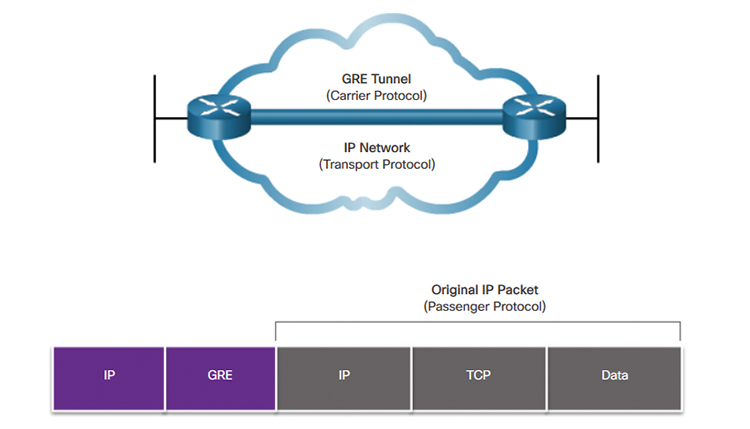
\includegraphics[width=0.75\linewidth]{tesi_stile/img/funzionamento_GRE.png}
    \caption{Funzionamento protocollo GRE con relativo pacchetto \cite{funzionamento_GRE_articolo}.}
    \label{funzionamento_GRE}
\end{figure}
Mirai dispone di due modalità di attacco che sfruttano il protocollo GRE le quali sono:
\begin{itemize}
    \item \textbf{GRE Ethernet flood (greeth)}: i bot inviano un grande volume di pacchetti GRE al server bersaglio. Il payload, in questo caso specifico, è un frame Ethernet con indirizzi MAC sorgente e destinazione casuali incapsulato all'interno di un pacchetto GRE. Il payload all'interno del frame Ethernet è un pacchetto UDP con indirizzi IP sorgente destinazione casuali;
    \item \textbf{GRE IP flood (greip)}: il meccanismo è lo stesso dell'attacco \emph{greeth} soltanto che in questo caso il payload è un pacchetto UDP con dati casuali incapsulato all'interno di un pacchetto GRE. Inoltre rispetto al greeth abbiamo un indicatore BPS più basso visto che i pacchetti sono più leggeri, di conseguenza quindi si ha un PPS più alto \cite{info_attacchi_mirai}.
\end{itemize}
\subsubsection{Altre tipologie di attacco }
Oltre ai vettori di attacco descritti precedentemente Mirai dispone di altre 3 metodologie di attacco di seguito descritte:
\begin{itemize}
    \item \textbf{VSE flood (vse)}: VSE (Valve Source Engine) è un motore grafico sviluppato dalla Valve Corporation. L'attacco VSE flood è un'estensione degli attacchi UDP, in particolare con l'attacco i bot inondano il \emph{Source Engine Query} in modo da interrompere la disponibilità di un server gaming bersaglio. Tutto ciò fa intuire che questo è un attacco pensato proprio per il mercato videoludico~\cite{info_attacchi_mirai}; 
    \item \textbf{DNS resolver flood (dns)}: con questa metodologia di attacco i bot inviano numerose richieste DNS di tipo \emph{A-record} al server ricorsivo bersaglio. Poiché il server non ha nella propria cache la risoluzione dei domini richiesti, è costretto a inoltrare ogni query al name server autoritativo. In questo modo sia il server ricorsivo sia il name server autoritativo vengono saturati di richieste, compromettendo la loro disponibilità \cite{info_attacchi_mirai}. Nella figura~\ref{spiegazione_dns_flood} viene illustrato il funzionamento di un attacco \emph{DNS resolver flood} nell'ambito della botnet Mirai;
    \begin{figure}[H]
        \centering
        \includegraphics[width=0.75\linewidth]{tesi_stile/img/spiegazione_dns_flood.png}
        \caption{DNS resolver flood in Mirai \cite{info_attacchi_mirai}.}
        \label{spiegazione_dns_flood}
    \end{figure}
    \item \textbf{HTTP flood (http)}: con questo vettore di attacco i bot inviano ripetutamente richieste HTTP ad un server web, quando il server web bersaglio non riesce più a rispondere a queste richieste si verifica un'interruzione della disponibilità per le richieste legittime.
    Nel caso di Mirai questo attacco risulta particolarmente versatile, poiché chi lo lancia può configurare diversi parametri, come il metodo HTTP, il dominio e il numero di connessioni.
\end{itemize}
La Tabella~\ref{attacchi_mirai} presenta un riepilogo dei 10 attacchi implementati da Mirai analizzati precedentemente.
\begin{table}[H]
    \centering
    \begin{tabular}{|c | c | c| c|}
        \hline
         \textbf{Attacco} & \textbf{ID} & \textbf{Comando} & \textbf{Livello OSI bersagliato} \\ \hline
         UDP flood & 0 & udp & Livello di trasporto  \\
         VSE flood & 1 & vse & Livello di applicazione\\
         DNS flood & 2 & dns & Livello di applicazione \\
         SYN flood & 3 & syn & Livello di trasporto \\
         ACK floog & 4 &ack & Livello di trasporto\\
         TCP STOMP flood & 5 & stomp & Livello di trasporto \\
         GRE IP flood & 6 & greip & Livello di rete \\
         GRE Ethernet flood & 7 & greeth & Livello di rete \\
         UDP flood con meno opzioni & 9 & udpplain & Livello di trasporto \\ 
         HTTP flood & 10 & http & Livello di applicazione \\
        \hline
    \end{tabular}
    \caption{Tipologie di attacco supportate da Mirai.}
    \label{attacchi_mirai}
\end{table}